\documentclass{beamer}
\mode<presentation>
% The Beamer class comes with a number of default slide themes
% which change the colors and layouts of slides. Below this is a list
% of all the themes, uncomment each in turn to see what they look like.
  %\usetheme{default}
  %\usetheme{AnnArbor}
  %\usetheme{Antibes}
  %\usetheme{Bergen}
  %\usetheme{Berkeley}
  %\usetheme{Berlin}
  %\usetheme{Boadilla}
  %\usetheme{CambridgeUS}
  %\usetheme{Copenhagen}
  %\usetheme{Darmstadt}
  %\usetheme{Dresden}
  %\usetheme{Frankfurt}
  %\usetheme{Goettingen}
  %\usetheme{Hannover}
  %\usetheme{Ilmenau}
  %\usetheme{JuanLesPins}
  %\usetheme{Luebeck}
  \usetheme{Madrid}
  %\usetheme{Malmoe}
  %\usetheme{Marburg}
  %\usetheme{Montpellier}
  %\usetheme{PaloAlto}
  %\usetheme{Pittsburgh}
  %\usetheme{Rochester}
  %\usetheme{Singapore}
  %\usetheme{Szeged}
  %\usetheme{Warsaw}

  % As well as themes, the Beamer class has a number of color themes
  % for any slide theme. Uncomment each of these in turn to see how it
  % changes the colors of your current slide theme.

  %\usecolortheme{albatross}
  %\usecolortheme{beaver}
  %\usecolortheme{beetle}
  %\usecolortheme{crane}
  %\usecolortheme{dolphin}
  %\usecolortheme{dove}
  %\usecolortheme{fly}
  %\usecolortheme{lily}
  %\usecolortheme{orchid}
  %\usecolortheme{rose}
  %\usecolortheme{seagull}
  %\usecolortheme{seahorse}
  %\usecolortheme{whale}
  %\usecolortheme{wolverine}
  %\setbeamertemplate{footline} % To remove the footer line in all slides uncomment this line
  %\setbeamertemplate{footline}[page number] % To replace the footer line in all slides with a simple slide count uncomment this line
  %\setbeamertemplate{navigation symbols}{} % To remove the navigation symbols from the bottom of all slides uncomment this line


  \usepackage{graphicx} % Allows including images
  \usepackage{booktabs} % Allows the use of \toprule, \midrule and \bottomrule in tables

  \title[Journal Club]{Transformation and differential abundance analysis of microbiome data incorporating phylogeny} % The short title appears at the bottom of every slide, the full title is only on the title page

  \author{Emily Palmer} % Your name
  \institute[OSU] % Your institution as it will appear on the bottom of every slide, may be shorthand to save space
  {Oregon State University \\ % Your institution for the title page
    \medskip
    \textit{palmerem@oregonstate.edu} % Your email address
  }
  \date{\today} % Date, can be changed to a custom date

  \begin{document}

  \begin{frame}
  \titlepage % Print the title page as the first slide
  \end{frame}

  % \begin{frame}
  % \frametitle{Overview} % Table of contents slide, comment this block out to remove it
  % \tableofcontents % Throughout your presentation, if you choose to use \section{} and \subsection{} commands, these will automatically be printed on this slide as an overview of your presentation
  % \end{frame}


  \begin{frame}
  \begin{figure}[!htb]
	\centering
	
\includegraphics[width=0.95\textwidth]{img/paper_title.png}
\end{figure}
\end{frame}

%----------------------------------------------------------------------------------------
\begin{frame}
\frametitle{Outline: Overview of paper}
 \begin{itemize}
   \item Extend Dirichlet-tree multinomial to zero-inflated Dirichlet tree multinomial to model multivariate microbial counts.
   \item Use an Empirical Bayes based posterior mean transformation to convert raw counts into non-zero relative abundances that sum to 1.
   \item Introduce phylogenetically informed DA procedure on transformed data - adaptive analysis of composition of microbiomes for DA testing (adaANCOM)- log-ratios adaptively on the tree for each taxon.
 \end{itemize}
\end{frame}
%----------------------------------------------------------------------------------------

%----------------------------------------------------------------------------------------
\section{Setting of method environment: Introduction}
\begin{frame}
\frametitle{Introduction}
   \begin{itemize}
     \item Differential abundance tests need to account for the high dimensional, sparse, compositional, negatively and positively correlated, phylogenetically structured microbiome data.
      \item Scaling methods to correct for compositional bias (TMM, DESeq, CSS) - assume that most taxa are not differentially abundant, when the count matrix is sparse it can over or underestimate diversity, distort correlations
      % TODO look over introduction again
   \end{itemize}
\end{frame}
%----------------------------------------------------------------------------------------
\section{Zero-inflated Dirichlet-tree multinomial (ZIDTM)}

%----------------------------------------------------------------------------------------
\begin{frame}
\frametitle{Review of Dirichlet-Multinomial distribution}
\begin{itemize}
  \item The Dirichlet-multinomial (DM) distribution is commonly used for OTU counts and is a compound distribution comprised of Dirichlet and Multinomial distributions
  % over-dispersed and compotiional
   % - compound multinomial with probabilities from a Dirichlet prior

  \item Let $\boldsymbol y = (y_1, \ldots , y_K)^T$ be the count vector for a sample with $K$ OTUs.

\item $y^+ = \sum_{k = 1}^K y_k, \boldsymbol p = (p_1, \ldots, p_K)^T$,  $\sum_{k = 1}^K p_k = 1, \alpha^+ = \sum_{k = 1}^K \alpha_k$
\begin{columns}[c] % The "c" option specifies centered vertical alignment while the "t" option is used for top vertical alignment

\column{.5\textwidth} % Left column and width
\begin{itemize}
  \item Multinomial pdf:
    \begin{figure}[!htb]
  	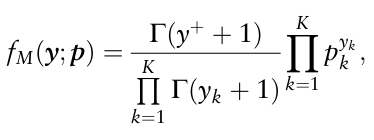
\includegraphics[width=0.65\textwidth]{img/multinomial_pdf.png}
    \end{figure}
\end{itemize}
\column{.5\textwidth} % Right column and width
\begin{itemize}
  \item Dirichlet pdf:
  \begin{figure}[!htb]
  	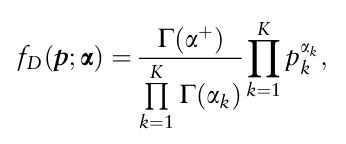
\includegraphics[width=0.65\textwidth]{img/dirichlet_pdf.png}
  \end{figure}
\end{itemize}
\end{columns}

\item Combining both we get the Dirichlet-Multinomial distribution:
\begin{figure}[!htb]
  \centering
  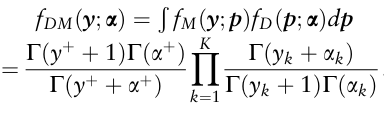
\includegraphics[width=0.5\textwidth]{img/dm_pdf.png}

\end{figure}

\end{itemize}
\end{frame}
%-----------------------------------------------------------

%----------------------------------------------------------------------------------------
\begin{frame}
\frametitle{Relationship between Gamma, Beta, \& Dirichlet distributions}
\begin{itemize}
  \item Let $Z_1, \ldots , Z_K$ independent $Z_k \sim \text{Gamma}(\alpha_k, \lambda)$,
  \item $X_k = \frac{Z_k}{\sum_{j=1}^K Z_j}$
  \item $W_k = \frac{Z_k}{\sum_{j = k}^K Z_j}$
  \item Joint distribution of $\boldsymbol X = (X_1, \ldots , X_K)^T$ is Dirichlet distributed with parameter $\boldsymbol \alpha$
  \item $W_k \sim \text{Beta}(\alpha_k, \alpha_k^+)$ independent
  \item $X_k = W_k \prod_{j=1}^{k-1}(1 - W_j)$
  \item We can rewrite the Dirichlet-Multinomial distribution as
  \begin{figure}[!htb]
	\centering
	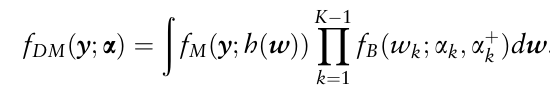
\includegraphics[width=0.6\textwidth]{img/dm_dist.png}
\end{figure}
\item $h(\cdot)$ is the transformation from $\boldsymbol W$ to $\boldsymbol X$.
\end{itemize}
\end{frame}
%----------------------------------------------------------------------------------------
%----------------------------------------------------------------------------------------
\begin{frame}
\frametitle{Zero Inflated Dirichlet Multinomial}
\begin{itemize}
  \item We can introduce zero inflation by defining the Zero Inflated Dirichlet Multinomial (ZIDM) as:
\begin{figure}[!htb]
	\centering
	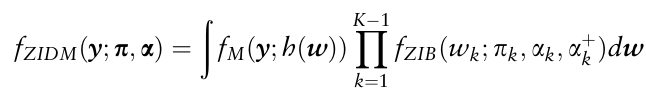
\includegraphics[width=0.75\textwidth]{img/zidm.png}
\end{figure}

\item where
\begin{figure}[!htb]
	\centering
	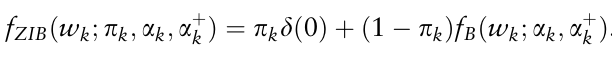
\includegraphics[width=0.75\textwidth]{img/zib.png}
\end{figure}
is a zero-inflated binomial distribution

\item $\pi_k$ is the probability of zero-inflation in the $k$th component $\delta(\cdot)$ is the Dirac delta function

\end{itemize}
\end{frame}
%----------------------------------------------------------------------------------------
%----------------------------------------------------------------------------------------
\begin{frame}
\frametitle{Introducing the Dirichlet Tree Multinomial}

\begin{itemize}
  \item Suppose the relationships between OTUs are encoded in a tree $\mathcal{T}$ which is composed of internal nodes $\mathcal{V}$ and leaf nodes $\mathcal{L}$
  \item Leaf nodes are OTUs, internal nodes are the node to branch on the phylogenetic tree
  \item For each $v \in \mathcal{V}$, denote $C_v$ as the set of child nodes of $v$, $\boldsymbol y_v$ the vector of counts correpsonding to $C_v$, and $y_v^+ = \sum_{u \in C_v} y_u$.

\end{itemize}

\end{frame}

\begin{frame}
\frametitle{Dirichlet Tree Multinomial \& Zero-Inflated Dirichlet Tree Multinomial}
\begin{itemize}
    \item Assume that $\boldsymbol y_v$ conditional on $y_v^+$ are independent across internal nodes, the Dirichlet Tree Multinomial (DTM) distribution is the product of DM distributions that factorize over the tree
    \begin{figure}[!htb]
  	\centering
  	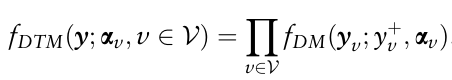
\includegraphics[width=0.55\textwidth]{img/dtm.png}
  \end{figure}

    \item To extend the DTM to the ZIDTM, we replace the Dirichlet multinomial with Zero-Inflated Dirichlet Multinomial

    \begin{figure}[!htb]
  	\centering
  	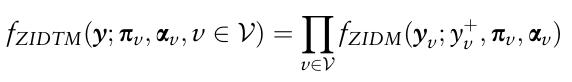
\includegraphics[width=0.7\textwidth]{img/zidtm.png}
  \end{figure}
  % \item The ZIDTM is a flexible distribution that accounts for over dispersion, data sparsity, inter-taxon structures & phylogenetic structure
\end{itemize}
\end{frame}
%----------------------------------------------------------------------------------------
%----------------------------------------------------------------------------------------
\begin{frame}
\frametitle{Example}
\begin{figure}[!htb]
	\centering
	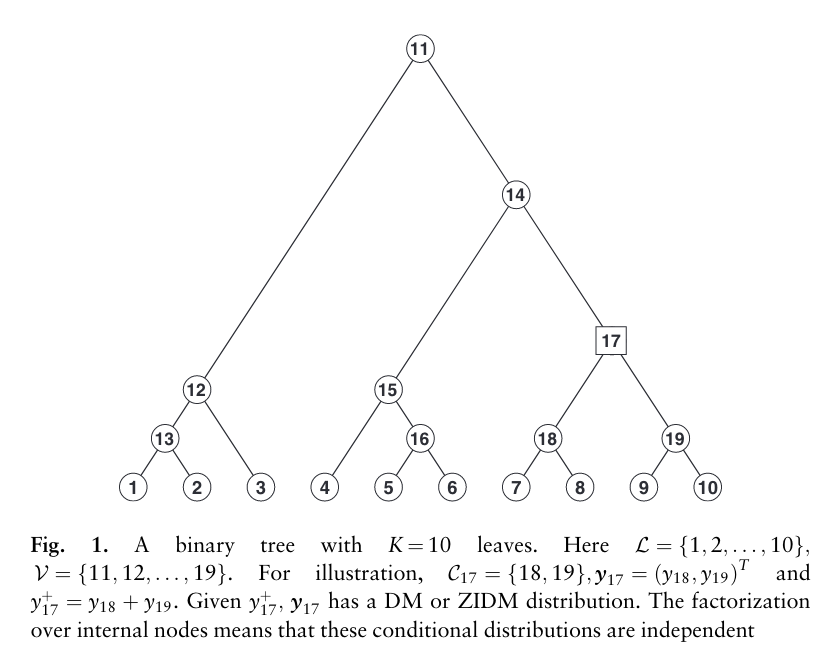
\includegraphics[width=0.85\textwidth]{img/tree_example.png}
\end{figure}
\begin{itemize}
  \item Unlike DM distributions, DTM and ZIDTM correlations between counts on tree nodes can be simultaneously negative and positive (WHY?)
\end{itemize}
\end{frame}


%----------------------------------------------------------------------------------------

%----------------------------------------------------------------------------------------
%----------------------------------------------------------------------------------------
\section{Maximum likelihood estimation for ZIDTM}

%----------------------------------------------------------------------------------------
\begin{frame}
\frametitle{Maximum likelihood estimation for ZIDTM}
\begin{itemize}
  \item Use EM-algorithm to estimate unknown parameters: $\boldsymbol\theta = \{\boldsymbol\alpha_v, \boldsymbol\pi_v, v \in \mathcal{V}\}$
  \item Assume $C_v = \{ 1,\ldots , K_v\}$, where $K_v = |C_v|$
  \item Consider $n$ observations $\boldsymbol y^1, \ldots , \boldsymbol y^n$, then the log-likelihood function (without constant terms) is:
  \begin{figure}[!htb]
	\centering
	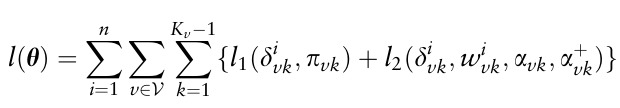
\includegraphics[width=0.65\textwidth]{img/log_liklihood.png}
\end{figure}
with
\begin{figure}[!htb]
	\centering
	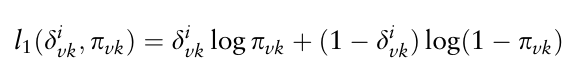
\includegraphics[width=0.55\textwidth]{img/l1.png}
\end{figure}

\begin{figure}[!htb]
	\centering
	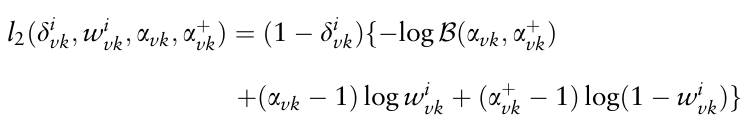
\includegraphics[width=0.65\textwidth]{img/l2.png}
\end{figure}
\item $\delta_{vk}^i$ is the indicator of zero-inflation $\mathcal{B}()$ is the beta function
\end{itemize}

\end{frame}
%----------------------------------------------------------------------------------------
%----------------------------------------------------------------------------------------
%----------------------------------------------------------------------------------------
\begin{frame}
\frametitle{E-step}
\begin{itemize}
  \item Compute expectation of $l(\boldsymbol\theta)$ with respect to posterior distribution of $(\delta_{vk}^i, w_{vk}^i)|\boldsymbol{y}_{v}^i$, indexed by current value of $\boldsymbol\theta$, which gives the $Q$-function:
  \begin{figure}[!htb]
	\centering
	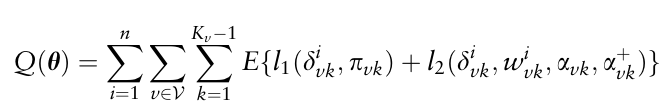
\includegraphics[width=0.75\textwidth]{img/q.png}
\end{figure}
\end{itemize}
\end{frame}
%----------------------------------------------------------------------------------------


%----------------------------------------------------------------------------------------
\begin{frame}
\frametitle{E-step: Definitions}
\begin{itemize}
  \item $\delta_{vk}^{i*} = E(\delta_{vk}^i|\boldsymbol{y}_v^i)$
  \item $R_{vk}^{i*} = E(\log w_{vk}^i|\boldsymbol{y}_v^i, \delta_{vk}^i = 0)$
  \item $S_{vk}^{i*} = E\{\log(1 - w_{vk}^i)|\boldsymbol{y}_{v}^i, \delta_{vk}^i = 0\}$
  \item Then,
\begin{figure}[!htb]
	\centering
	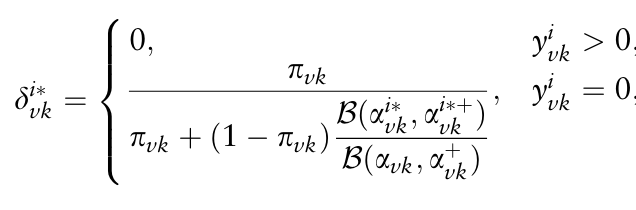
\includegraphics[width=0.55\textwidth]{img/deltastar.png}
\end{figure}


\begin{columns}[c]
  \column{.5\textwidth}
  \begin{figure}[!htb]
	\centering
	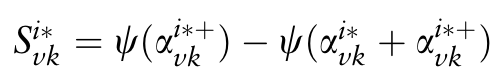
\includegraphics[width=0.75\textwidth]{img/sstar.png}
\end{figure}
  \column{.5\textwidth}
  \begin{figure}[!htb]
  	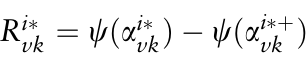
\includegraphics[width=0.55\textwidth]{img/rstar.png}
  \end{figure}
\end{columns}
\item $\alpha_{vk}^{i*} = \alpha_{vk} + y_{vk}^i,\quad  \alpha_{vk}^{i*+} = \sum_{j = k+1}^{K_v}\alpha_{vk}^{i*}, \quad \psi(\cdot)$ is the digamma function.

\end{itemize}
\end{frame}
%----------------------------------------------------------------------------------------
%----------------------------------------------------------------------------------------
\begin{frame}
\frametitle{E-step: Q-function}
\begin{itemize}
  \item We can rewrite $Q(\boldsymbol\theta)$ as:
  \begin{figure}[!htb]
	\centering
	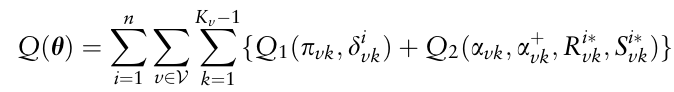
\includegraphics[width=0.65\textwidth]{img/qfun2.png}
\end{figure}
\item where
\begin{figure}[!htb]
	\centering
	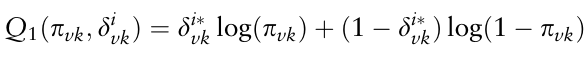
\includegraphics[width=0.65\textwidth]{img/q1.png}
\end{figure}
and
\begin{figure}[!htb]
	\centering
	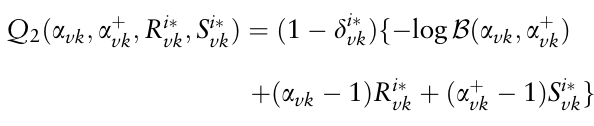
\includegraphics[width=0.65\textwidth]{img/q2.png}
\end{figure}
\end{itemize}
\end{frame}
%----------------------------------------------------------------------------------------
%----------------------------------------------------------------------------------------
\begin{frame}
\frametitle{M-step}
\begin{itemize}
  \item Maximize $Q(\boldsymbol\theta)$ with respect to $\boldsymbol\theta$
  \item The parameters in $Q_1$ and $Q_2$ can be optimized separately
  \item Model depends on ordering of OTUs at each internal node (matching problem)
  \item Fit separate ZIDM model for each possible ordering of $|C_v|$ taxa, and select the best fitted model.
  \item Computational cost is
  $O(\sum_{v \in \mathcal{V}}|C_v|!)$
  compared to $O(|\mathcal{L}|!)$ for GDM or ZIDM models
\end{itemize}
\end{frame}
%----------------------------------------------------------------------------------------
%----------------------------------------------------------------------------------------
%----------------------------------------------------------------------------------------
\begin{frame}
\frametitle{Binary trees }
\begin{itemize}
     \item From now on, consider binary trees
     \item i.e. $|C_v| = 2$ for all $v \in \mathcal{V}$
     \item Dirichlet, multinomial, dirichlet multinomial, and zero inflated dirichlet multinomial are reduced to beta, binomial, beta-binomial and zero-inflated beta-binomial.
     \item The ZIDTM is then a product of ZIBBs
\end{itemize}
\end{frame}
%----------------------------------------------------------------------------------------
%----------------------------------------------------------------------------------------


\begin{frame}
 \frametitle{Posterior mean transformation}
 \begin{itemize}
   \item Estimate underlying proportions from Bayesian perspective (since Dirichlet is conjugate to multinomial)
   \item Consider the posterior mean for the Dirichlet Multinomial:
   \begin{figure}[!htb]
 	\centering
 	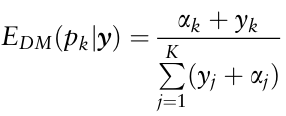
\includegraphics[width=0.35\textwidth]{img/edm.png}
 \end{figure}
 \item We estimate unknown parameters by maximizing data likelihood
 \item Use the estimated parameters as "pseudo data" and combine with real observed data.
 \item This produces non-zero proportions for zero counts
 \item Alternative to using a pseudo-count for sample proportions
 \item Becomes difficult in presence of zero-inflation
 \end{itemize}

\end{frame}

%----------------------------------------------------------------------------------------
\begin{frame}
\frametitle{Solving posterior mean transformation}
\begin{itemize}
  \item When we have a binary tree, there is an explicit closed-form solution to the zero-inflation
  \item At each internal node $v \in \mathcal{V}$,
  \begin{figure}[!htb]
	\centering
	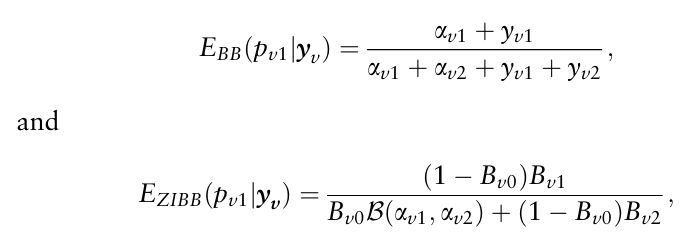
\includegraphics[width=0.65\textwidth]{img/ebbzib.png}
  \end{figure}
  \begin{itemize}
    \item $B_{v0} = \pi I(y_{v1} = 0)$
    \item $B_1 = \mathcal{B}(1 + \alpha_{v1} + y_{v1}, \alpha_{v2} + y_{v2})$
    \item $B_2 = \mathcal{B}(\alpha_{v1} + y_{v1}, \alpha_{v2} + y_{v2})$
  \end{itemize}

\end{itemize}
\end{frame}
%----------------------------------------------------------------------------------------

%----------------------------------------------------------------------------------------
\begin{frame}
\frametitle{Likelihood-ratio test \& count transformation}
\begin{itemize}
  \item Having a correct model specification at internal nodes effects quality of posterior estimates.
  \item Perform a two-stage likelihood-ratio test
  \item First, assume count data at $v \in \mathcal{V}$ are not zero-inflated, fit beta-binomial model and test for over-dispersion.
  \item Counts at nodes without over-dispersion are transformed into sample proportions after adding constant of .5, equivalent to using $E_{BB}$ with $\alpha_{v1} = \alpha_{v2} = 0.5$
  \item Second, Nodes with over-dispersion are refit using a ZIBB model, and tested again for zero-inflation
  \item Counts are then transformed using $E_{ZIBB}(p_{v1}|\boldsymbol y_v)$.
  \item If there is no zero-inflation,  counts are transformed using $E_{BB}(p_{v1}, \boldsymbol y_v)$
  \item $\hat{\boldsymbol p}_v = (\hat p_{v1}, 1 - \hat{p}_{v1})^T$ is the posterior estimate

\end{itemize}
\end{frame}
%----------------------------------------------------------------------------------------
%----------------------------------------------------------------------------------------
\begin{frame}
\frametitle{Path-level definitions - Phylogeny-aware normalization }
\begin{itemize}
  \item To ensure that the normalization is 'phylogeny-aware', we consider the path level instead of focussing on individual internal nodes.
  \item Define $\mathcal{A}_u$ as the ancestor node set of $u$ for each node $u \in \mathcal{L} \cup \mathcal{V}$ that contains all internal nodes in the path from the root node to $u$
  \item $\mathcal{L}_u$ is the set of leaves in the same path
  \begin{columns}[c] % The "c" option specifies centered vertical alignment while the "t" option is used for top vertical alignment

  \column{.45\textwidth} % Left column and width
  \begin{itemize}
    \item $\mathcal{A}_1 = \mathcal{A}_2 = \{11,12,13\}$, $\mathcal{A}_3 = \{11,12\}$, $\mathcal{L}_{11} = \mathcal{L}, \mathcal{L}_{12} = \{1,2,3\}, \mathcal{L}_{13} = \{1,2\}$
  \end{itemize}

  \column{.5\textwidth} % Right column and width
  \begin{figure}[!htb]
  	\centering
  	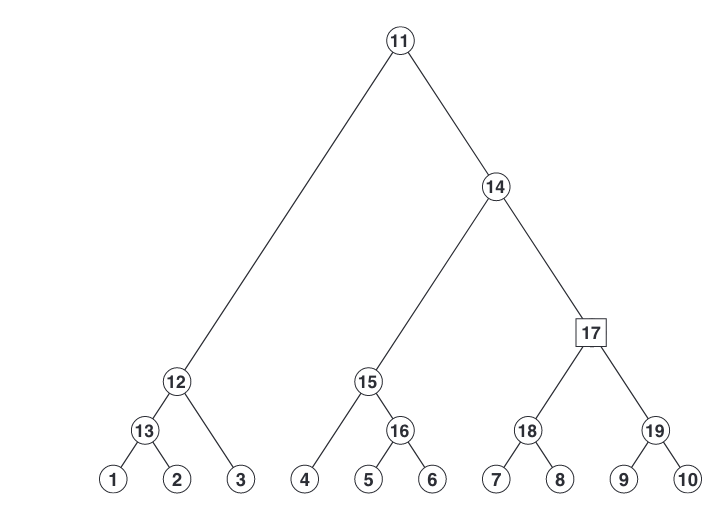
\includegraphics[width=0.65\textwidth]{img/ex2.png}
  \end{figure}

  \end{columns}
  \item Define $q_u = \prod_{v \in \mathcal{A}_u}\hat p_v$
  \item $\mathcal{U}$ is the set of nodes such that $\cup_{u \in U} \mathcal{L}_u = \mathcal{L}$, $\mathcal{L}_u \cap \mathcal{L}_{u'} = \emptyset$ when $u \neq u'$.
  \item Then, $\sum_{u \in \mathcal{U}} q_u = 1$ and $\sum_{l \in \mathcal{L}} q_l = 1$
\end{itemize}
\end{frame}
%----------------------------------------------------------------------------------------
\section{adaANCOM}

%----------------------------------------------------------------------------------------
\begin{frame}
\frametitle{adaANCOM}
\begin{itemize}
  \item Detect differentially abundant OTUs at ecosystem level
  \item Similar to ANCOM
  \item Difference is how we use the phylogenetic tree to incorporate this information
  \item Tests differences between two groups
  \item Speed up ANCOM by using phylogenetic tree to construct adaptive log-ratios
\end{itemize}
\end{frame}
%----------------------------------------------------------------------------------------
%----------------------------------------------------------------------------------------
\begin{frame}
\frametitle{Hypothesis tests - ANCOM}
\begin{itemize}
  \item Test the hypothesis
  $$H_{0l}: \log \mu_l^1 = \log \mu_l^2$$
  for $l \in \mathcal{L} = \{1, \ldots , K\}$, and where $\mu_l^g$ is the mean absolute abundance of the $l$th OTU from $g$th group, and $g = 1,2$
  \item In ANCOM, we test $K-1$ hypothesis using each OTU as the denominator in the additive log ratio
  $$H_{0lm}: \log(\mu_l^1/\mu_m^1) = \log(\mu_l^2/\mu_m^2)$$ for all $m \neq l$
  \item ANCOM counts the number of rejections across the $K-1$ hypothesis tests, and compares to the empirical distribution of counts to determine if the $l$th OTU is differentially abundant.
  \item If $K$ is high, ANCOM suffers from a high FDR. Additionaly the computational burden is high
\end{itemize}
\end{frame}
%----------------------------------------------------------------------------------------
%----------------------------------------------------------------------------------------
\begin{frame}
\frametitle{adaANCOM log-ratios \& hypothesis tests}
\begin{itemize}
  % \item Make log-ratios adaptively by using the phylogenetic tree
  \item Assume that abundance difference on the log scale at an internal node is passed down to child nodes
  \item adaANCOM is comprised of a two-step process
  \begin{enumerate}
    \item Test the internal node-level hypothesis
    \begin{figure}[!htb]
	\centering
	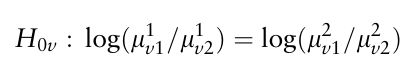
\includegraphics[width=0.4\textwidth]{img/internalh0.png}
\end{figure}
for $v \in \mathcal{V}$, with $\mu_{v1}^g$ and $\mu_{v2}^g$ as mean absolute abundances of children of $v$ from the $g$th group.

 For a given $\alpha$,$\mathcal{D}_{\mathcal{V}}$ is the set of internal nodes which the hypotheses are rejected

 \item For each leaf node $l \in \mathcal{L}$, calculate the log-ratio

  Define $ref_l$ as the sibling node of $l$ if $\mathcal{A}_l \cap \mathcal{D}_{\mathcal{V}} = \emptyset$ and the child node of $v$ not in $\mathcal{A}_l$ otherwise, when $v$ is the node in $\mathcal{A}_l \cap \mathcal{D}_{\mathcal{V}}$ closest to the root node.

   The null hypothesis is:
   \begin{figure}[!htb]
	\centering
	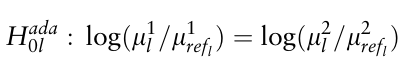
\includegraphics[width=0.4\textwidth]{img/h0ref.png}
  \end{figure}


  \end{enumerate}
  \item  adaANCOM rejects the null hypothesis $H_{0l}$ if $H_{0l}^{ada}$ is rejected
\end{itemize}
\end{frame}
%----------------------------------------------------------------------------------------

%----------------------------------------------------------------------------------------
\begin{frame}
\frametitle{adaANCOM example}

\begin{columns}[c] % The "c" option specifies centered vertical alignment while the "t" option is used for top vertical alignment

\column{.45\textwidth} % Left column and width
\begin{itemize}
  \item Assume $\mathcal{D}_{\mathcal{V}} = 17$.
  \item $ref_1 = 2, ref_2 = 1$

  $ ref_3 = 13, ref_4 = 16, $

  $ref_5 = 6, ref_6 = 5,$

  $ ref_7 = ref_8 = 19, $

  $ref_9 = ref_{10} = 18$
\end{itemize}

\column{.5\textwidth} % Right column and width
\begin{figure}[!htb]
	\centering
	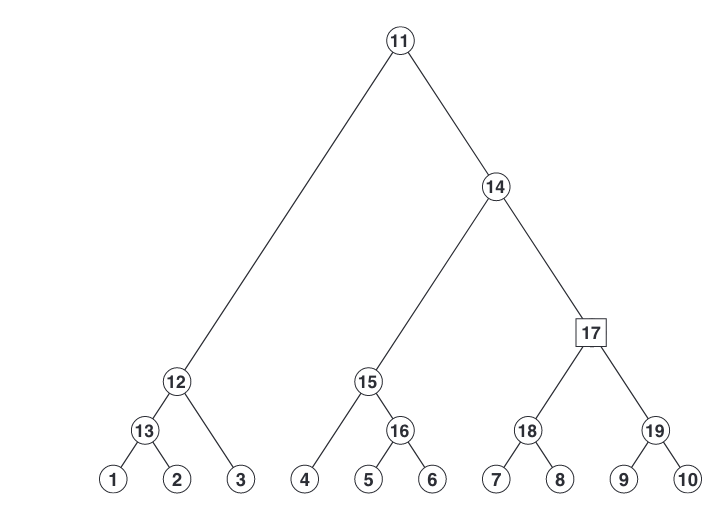
\includegraphics[width=0.95\textwidth]{img/ex2.png}
\end{figure}

\end{columns}
\end{frame}
%----------------------------------------------------------------------------------------
%----------------------------------------------------------------------------------------
\begin{frame}
\frametitle{Accounting for log-ratios of zero $y_u$ counts}
\begin{itemize}
  \item $H_{0v}$ and $H_{0l}^{ada}$ are based on the log-ratios of $q_u$s for $u \in \mathcal{L} \cup \mathcal{V}$, but when the original $y_u$ counts have many zero counts, log-ratios give abnormal results, and test statistics are sensitive to these abnormal values
  \item For internal node $v$, define $\phi_v $ as the maximum of $$|\log(\hat p_{v1}/\hat p_{v2})|$$  that have $y_{v1} > 0$ and $y_{v2} > 0$.
  \item Data with $y_{v1} = 0$ or $y_{v2} = 2$ are removed if $|\log(\hat p_{v1}/\hat p_{v2})| > \phi_v$
\end{itemize}
\end{frame}
%----------------------------------------------------------------------------------------

%----------------------------------------------------------------------------------------
\begin{frame}
\frametitle{Comparisons to ANCOM}
\begin{itemize}
  \item Similar to ANCOM, adaANCOM uses relative abundance data, constructs log-ratios, and performs t-tests or Wilcoxon-rank-sum tests.
  \item The advantage of adaANCOM is the computation time, as the number of tests is reduced by a factor of $|\mathcal{L}|$.
  \item adaANCOM also has an advantage of interpretability since we are guided by the tree, so we result in both DA leaves and nodes.
  \item Additionally, adaANCOM controls FDR better
\end{itemize}
\end{frame}
%----------------------------------------------------------------------------------------

%----------------------------------------------------------------------------------------
\begin{frame}
\frametitle{adaANCOM algorithm}
\begin{figure}[!htb]
	\centering
	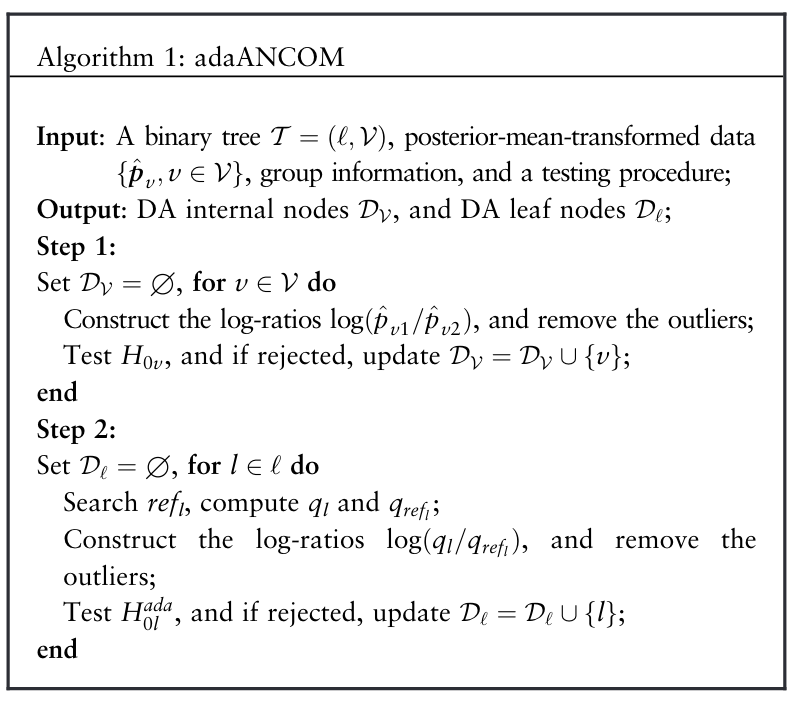
\includegraphics[width=0.75\textwidth]{img/algorithm.png}
	\caption{}
	\label{}
\end{figure}
\end{frame}
%----------------------------------------------------------------------------------------


  \end{document}
